\documentclass{article}

\usepackage[preprint]{neurips_2025}
\usepackage[utf8]{inputenc} % allow utf-8 input
\usepackage[T1]{fontenc}    % use 8-bit T1 fonts
\usepackage{hyperref}       % hyperlinks
\usepackage{url}            % simple URL typesetting
\usepackage{booktabs}       % professional-quality tables
\usepackage{amsfonts}       % blackboard math symbols
\usepackage{nicefrac}       % compact symbols for 1/2, etc.
\usepackage{microtype}      % microtypography
\usepackage{xcolor}         % colors
\usepackage{graphicx} % Add Images


\title{Breaking News: An LLM Agent to Detect Bias in News}

\author{%
  Daniel Leniz\\
  Department of Computer Science\\
  University of South Florida\\
  Tampa, FL 33647 \\
  \texttt{dleniz@usf.edu} \\
  \And
  Louis-Marie Mondesir\\
  Department of Computer Science\\
  University of South Florida\\
  Tampa, FL 33647 \\
  \texttt{lmondesir1@usf.edu} \\
  \And
  Robert Malloy\\
  Department of Computer Science\\
  University of South Florida\\
  Tampa, FL 33647 \\
  \texttt{rmalloy1@usf.edu} \\
}


\begin{document}


\maketitle


\begin{abstract}
  The abstract paragraph should be indented \nicefrac{1}{2}~inch (3~picas) on
  both the left- and right-hand margins. Use 10~point type, with a vertical
  spacing (leading) of 11~points.  The word \textbf{Abstract} must be centered,
  bold, and in point size 12. Two line spaces precede the abstract. The abstract
  must be limited to one paragraph.
\end{abstract}


\section{Introduction}

This section is the introduction.


\subsection{Our Problem}

We would like to have an ai summarize and detect bias in news articles


\subsection{Our Approach}

We are going to develop an LLM agent to do this.


\section {Related Work}

This section introduces Related Work. 

\section{System Design}

This section introduces system design. Add pic here

\begin{figure}[t]
  \centering
  % either of these works:
  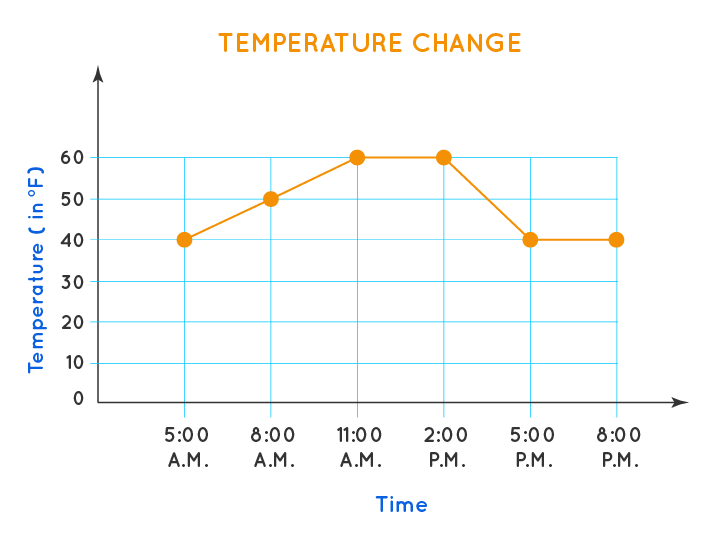
\includegraphics[width=0.9\linewidth]{figures/example.png}
  \caption{Overview of the system architecture used for bias detection and summarization.}
  \label{fig:system-arch}
\end{figure}


\subsection{qBias Dataset} 

Explain Bias Detector


\subsection{Bias Detector} 

Explain Bias Detector


\subsection{LLM Summarizer} 

Explain LLM Summarizer


\subsection{News Bias API and UI}  

Explain the News Bias work


\section{Evaluation}

This section is the evaluation.


\subsection{Midterm}

This section is midterm evaluation.


\subsection{Final}

This section is final Evaluation.


\section{Conclusion}

This section is the conclusion


\section{Acknowledgment}

\begin{itemize}
  \item \textbf{Daniel Leniz} (\textit{XX\%}) – Evaluation on Daniel
  \item \textbf{Louis-Marie Modesir} (\textit{XX\%}) – Evaluation on Louis
  \item \textbf{Robert Malloy} (\textit{XX\%}) – Evaluation on Robert
\end{itemize}

\bibliographystyle{plainnat}
\bibliography{references}

\end{document}